\newpage
\section{Checklists}\label{sec:Checklist}

%\begin{landscape}

The Pre-Launch Checklist will be taken care of by two team members. One of them will be responsible of reading out loud each item and marking them when they are done. The other one will be responsible for performing the stated actions. At the same time, the one reading will check that the actions are properly conducted. 

For three key actions (M5, M9 and M13), a third team member will be responsible of asking and, when possible, checking, that they have been properly conducted. 

\subsection{Pre-Launch Checklist}\label{sec:appL}



\begin{longtable} {|m{0.1\textwidth}|m{0.8\textwidth}|m{0.1\textwidth}|}
\hline
\textbf{ID} & \textbf{ITEM} & \textbf{CHECK} \\
\hline
\multicolumn{2}{|l|}{ \textbf{SCIENCE} } & \\
\hline
& \textbf{CAC} & \\
\hline
S1 & Remove the CAC wall with the D-SUB connector, if it's not removed already. & \\ \hline
S2 & Connect picarro to quick connector stem at No 10. & \\ \hline
S3 & Attach the fill gas bottle's quick connector stem to quick connector body No 1. & \\ \hline
S4 & Let the fill gas run through the AirCore at a flow rate of 40ml/min. & \\ \hline
S5 & Leave it flushing over night. & \\ \hline
S6 & Detach quick connector stem at No 1. & \\ \hline
S7 & Detach the quick connector stem at No 10. & \\ \hline
S8 & Disconnect the picarro analyser. & \\ \hline
S9 & Connect the dryer tube No 14 to No 13. & \\ \hline
S10 & Connect parts 11 to 21. & \\ \hline
S11 & Check all connections are tighten. & \\ \hline
S12 & Close the CAC's solenoid valve No 17. & \\ \hline
S13 & Connect quick connector stem No 10 to No 9. & \\ \hline
S14 & Connect No 10 with No 11. & \\ \hline
S15 & Check all connections are tighten. & \\ \hline
S16 & Put the CAC wall with the D-SUB connector back. & \\ \hline
& \textbf{AAC/MANIFOLD} & \\ \hline
S17 & Unscrew the plug from the inlet (1) and outlet tube (29). & \\ \hline
S18 & Screw in the male threaded quick connector to the inlet tube (1). & \\ \hline
S19 & Connect the vacuum pump and the dry gas bottle through a central valve to the AAC's inlet tube (1). & \\ \hline
S20 & Open flushing valve (27). & \\ \hline
S21 & Turn central valve on so that is open to dry gas. & \\ \hline
S22 & Let the dry gas run through the AAC's manifold for 10 minutes. & \\ \hline
S23 & Close flushing valve (27) & \\ \hline
S24 & Turn central valve off so that is close to dry gas. & \\ \hline
S25 & Disconnect the vacuum pump and the dry gas bottle through a central valve from the AAC's inlet tube (1). & \\ \hline
S26 & Screw in the plug to the AAC inlet tube (1). & \\ \hline
& \textbf{AAC/TUBES/BAGS} & \\ \hline
S27 & Connect the vacuum pump and the dry gas bottle through a central valve to the AAC's outlet tube (29). & \\ \hline
S28 & Make sure the AAC's inlet tube (1) is shielded. & \\ \hline
S29 & Open 1st bag's manual valve. & \\ \hline
S30 & Open flushing valve (27). & \\ \hline
S31 & Open 1st bag's solenoid valve in the manifold (23) & \\ \hline
S32 & Open central valve so that is open to dry gas. & \\ \hline
S33 & Start filling the bag with 3L of dry gas with a flow rate of 2L/min for 1.5 minutes. & \\ \hline
S34 & After 1.5 mins, when the bag is full, turn the central valve open to the vacuum , allowing the bag to empty. & \\ \hline
S35 & Empty the bag with controlled vacuum only 1-2 mbar below ambient pressure. & \\ \hline
S36 & Turn the central valve open to dry gas. & \\ \hline
S37 & Start filling the bag with 3L of dry gas with a flow rate of 2L/min for 1.5 minutes. & \\ \hline
S38 & After 1.5 mins, when the bag is full, turn the central valve open to the vacuum , allowing the bag to empty. & \\ \hline
S39 & Empty the bag with controlled vacuum only 1-2 mbar below ambient pressure. & \\ \hline
S40 & Repeat steps S36 to S39 one more time. & \\ \hline
S41 & Close 1st bag's solenoid valve in the manifold (23). & \\ \hline
S42 & Disconnect the vacuum pump and the dry gas bottle through a central valve from the AAC's outlet tube (29). & \\ \hline
S43 & Unscrew the plug from the AAC inlet tube (1). & \\ \hline
S44 & Connect the vacuum pump and the dry gas bottle through a central valve to the AAC's inlet tube (1). & \\ \hline
S45 & Turn central valve on so that is open to dry gas. & \\ \hline
S46 & Let the dry gas run through the AAC's manifold for 2 minutes. & \\ \hline
S47 & Close flushing valve (27) & \\ \hline
S48 & Turn central valve off so that is close to dry gas. & \\ \hline
S49 & Disconnect the vacuum pump and the dry gas bottle through a central valve from the AAC's inlet tube (1). & \\ \hline
S50 & Screw in the plug to the AAC inlet tube (1). & \\ \hline
S51 & Connect the vacuum pump and the dry gas bottle through a central valve to the AAC's outlet tube (29). & \\ \hline
S52 & Make sure the AAC's inlet tube (1) is shielded. & \\ \hline
S53 & Open 2nd bag's manual valve. & \\ \hline
S54 & Open flushing valve (27). & \\ \hline
S55 & Open 2nd bag's solenoid valve in the manifold (23) & \\ \hline
S56 & Open central valve so that is open to dry gas. & \\ \hline
S57 & Start filling the bag with 3L of dry gas with a flow rate of 2L/min for 1.5 minutes. & \\ \hline
S58 & After 1.5 mins, when the bag is full, turn the central valve open to the vacuum , allowing the bag to empty. & \\ \hline
S59 & Empty the bag with controlled vacuum only 1-2 mbar below ambient pressure. & \\ \hline
S60 & Turn the central valve open to dry gas. & \\ \hline
S61 & Start filling the bag with 3L of dry gas with a flow rate of 2L/min for 1.5 minutes. & \\ \hline
S62 & After 1.5 mins, when the bag is full, turn the central valve open to the vacuum , allowing the bag to empty. & \\ \hline
S63 & Empty the bag with controlled vacuum only 1-2 mbar below ambient pressure. & \\ \hline
S64 & Repeat steps S60 to S63 one more time. & \\ \hline
S65 & Close 2nd bag's solenoid valve in the manifold (23). & \\ \hline
S66 & Disconnect the vacuum pump and the dry gas bottle through a central valve from the AAC's outlet tube (29). & \\ \hline
S67 & Unscrew the plug from the AAC inlet tube (1). & \\ \hline
S68 & Connect the vacuum pump and the dry gas bottle through a central valve to the AAC's inlet tube (1). & \\ \hline
S69 & Turn central valve on so that is open to dry gas. & \\ \hline
S70 & Let the dry gas run through the AAC's manifold for 2 minutes. & \\ \hline
S71 & Close flushing valve (27) & \\ \hline
S72 & Turn central valve off so that is close to dry gas. & \\ \hline
S73 & Disconnect the vacuum pump and the dry gas bottle through a central valve from the AAC's inlet tube (1). & \\ \hline
S74 & Screw in the plug to the AAC inlet tube (1). & \\ \hline
S75 & Connect the vacuum pump and the dry gas bottle through a central valve to the AAC's outlet tube (29). & \\ \hline
S76 & Make sure the AAC's inlet tube (1) is shielded. & \\ \hline
S77 & Open 3rd bag's manual valve. & \\ \hline
S78 & Open flushing valve (27). & \\ \hline
S79 & Open 3rd bag's solenoid valve in the manifold (23) & \\ \hline
S80 & Open central valve so that is open to dry gas. & \\ \hline
S81 & Start filling the bag with 3L of dry gas with a flow rate of 2L/min for 1.5 minutes. & \\ \hline
S82 & After 1.5 mins, when the bag is full, turn the central valve open to the vacuum , allowing the bag to empty. & \\ \hline
S83 & Empty the bag with controlled vacuum only 1-2 mbar below ambient pressure. & \\ \hline
S84 & Turn the central valve open to dry gas. & \\ \hline
S85 & Start filling the bag with 3L of dry gas with a flow rate of 2L/min for 1.5 minutes. & \\ \hline
S86 & After 1.5 mins, when the bag is full, turn the central valve open to the vacuum , allowing the bag to empty. & \\ \hline
S87 & Empty the bag with controlled vacuum only 1-2 mbar below ambient pressure. & \\ \hline
S88 & Repeat steps S84 to S87 one more time. & \\ \hline
S89 & Close 3rd bag's solenoid valve in the manifold (23). & \\ \hline
S90 & Disconnect the vacuum pump and the dry gas bottle through a central valve from the AAC's outlet tube (29). & \\ \hline
S91 & Unscrew the plug from the AAC inlet tube (1). & \\ \hline
S92 & Connect the vacuum pump and the dry gas bottle through a central valve to the AAC's inlet tube (1). & \\ \hline
S93 & Turn central valve on so that is open to dry gas. & \\ \hline
S94 & Let the dry gas run through the AAC's manifold for 2 minutes. & \\ \hline
S95 & Close flushing valve (27) & \\ \hline
S96 & Turn central valve off so that is close to dry gas. & \\ \hline
S97 & Disconnect the vacuum pump and the dry gas bottle through a central valve from the AAC's inlet tube (1). & \\ \hline
S98 & Screw in the plug to the AAC inlet tube (1). & \\ \hline
S99 & Connect the vacuum pump and the dry gas bottle through a central valve to the AAC's outlet tube (29). & \\ \hline
S100 & Make sure the AAC's inlet tube (1) is shielded. & \\ \hline
S101 & Open 4th bag's manual valve. & \\ \hline
S102 & Open flushing valve (27). & \\ \hline
S103 & Open 4th bag's solenoid valve in the manifold (23) & \\ \hline
S104 & Open central valve so that is open to dry gas. & \\ \hline
S105 & Start filling the bag with 3L of dry gas with a flow rate of 2L/min for 1.5 minutes. & \\ \hline
S106 & After 1.5 mins, when the bag is full, turn the central valve open to the vacuum , allowing the bag to empty. & \\ \hline
S107 & Empty the bag with controlled vacuum only 1-2 mbar below ambient pressure. & \\ \hline
S108 & Turn the central valve open to dry gas. & \\ \hline
S109 & Start filling the bag with 3L of dry gas with a flow rate of 2L/min for 1.5 minutes. & \\ \hline
S110 & After 1.5 mins, when the bag is full, turn the central valve open to the vacuum , allowing the bag to empty. & \\ \hline
S111 & Empty the bag with controlled vacuum only 1-2 mbar below ambient pressure. & \\ \hline
S112 & Repeat steps S108 to S111 one more time. & \\ \hline
S113 & Close 4th bag's solenoid valve in the manifold (23). & \\ \hline
S114 & Disconnect the vacuum pump and the dry gas bottle through a central valve from the AAC's outlet tube (29). & \\ \hline
S115 & Unscrew the plug from the AAC inlet tube (1). & \\ \hline
S116 & Connect the vacuum pump and the dry gas bottle through a central valve to the AAC's inlet tube (1). & \\ \hline
S117 & Turn central valve on so that is open to dry gas. & \\ \hline
S118 & Let the dry gas run through the AAC's manifold for 2 minutes. & \\ \hline
S119 & Close flushing valve (27) & \\ \hline
S120 & Turn central valve off so that is close to dry gas. & \\ \hline
S121 & Disconnect the vacuum pump and the dry gas bottle through a central valve from the AAC's inlet tube (1). & \\ \hline
S122 & Screw in the plug to the AAC inlet tube (1). & \\ \hline
S123 & Connect the vacuum pump and the dry gas bottle through a central valve to the AAC's outlet tube (29). & \\ \hline
S124 & Make sure the AAC's inlet tube (1) is shielded. & \\ \hline
S125 & Open 5th bag's manual valve. & \\ \hline
S126 & Open flushing valve (27). & \\ \hline
S127 & Open 5th bag's solenoid valve in the manifold (23) & \\ \hline
S128 & Open central valve so that is open to dry gas. & \\ \hline
S129 & Start filling the bag with 3L of dry gas with a flow rate of 2L/min for 1.5 minutes. & \\ \hline
S130 & After 1.5 mins, when the bag is full, turn the central valve open to the vacuum , allowing the bag to empty. & \\ \hline
S131 & Empty the bag with controlled vacuum only 1-2 mbar below ambient pressure. & \\ \hline
S132 & Turn the central valve open to dry gas. & \\ \hline
S133 & Start filling the bag with 3L of dry gas with a flow rate of 2L/min for 1.5 minutes. & \\ \hline
S134 & After 1.5 mins, when the bag is full, turn the central valve open to the vacuum , allowing the bag to empty. & \\ \hline
S135 & Empty the bag with controlled vacuum only 1-2 mbar below ambient pressure. & \\ \hline
S136 & Repeat steps S132 to S135 one more time. & \\ \hline
S137 & Close 5th bag's solenoid valve in the manifold (23). & \\ \hline
S138 & Disconnect the vacuum pump and the dry gas bottle through a central valve from the AAC's outlet tube (29). & \\ \hline
S139 & Unscrew the plug from the AAC inlet tube (1). & \\ \hline
S140 & Connect the vacuum pump and the dry gas bottle through a central valve to the AAC's inlet tube (1). & \\ \hline
S141 & Turn central valve on so that is open to dry gas. & \\ \hline
S142 & Let the dry gas run through the AAC's manifold for 2 minutes. & \\ \hline
S143 & Close flushing valve (27) & \\ \hline
S144 & Turn central valve off so that is close to dry gas. & \\ \hline
S145 & Disconnect the vacuum pump and the dry gas bottle through a central valve from the AAC's inlet tube (1). & \\ \hline
S146 & Screw in the plug to the AAC inlet tube (1). & \\ \hline
S147 & Connect the vacuum pump and the dry gas bottle through a central valve to the AAC's outlet tube (29). & \\ \hline
S148 & Make sure the AAC's inlet tube (1) is shielded. & \\ \hline
S149 & Open 6th bag's manual valve. & \\ \hline
S150 & Open flushing valve (27). & \\ \hline
S151 & Open 6th bag's solenoid valve in the manifold (23) & \\ \hline
S152 & Open central valve so that is open to dry gas. & \\ \hline
S153 & Start filling the bag with 3L of dry gas with a flow rate of 2L/min for 1.5 minutes. & \\ \hline
S154 & After 1.5 mins, when the bag is full, turn the central valve open to the vacuum , allowing the bag to empty. & \\ \hline
S155 & Empty the bag with controlled vacuum only 1-2 mbar below ambient pressure. & \\ \hline
S156 & Turn the central valve open to dry gas. & \\ \hline
S157 & Start filling the bag with 3L of dry gas with a flow rate of 2L/min for 1.5 minutes. & \\ \hline
S158 & After 1.5 mins, when the bag is full, turn the central valve open to the vacuum , allowing the bag to empty. & \\ \hline
S159 & Empty the bag with controlled vacuum only 1-2 mbar below ambient pressure. & \\ \hline
S160 & Repeat steps S156 to S159 one more time. & \\ \hline
S161 & Close 6th bag's solenoid valve in the manifold (23). & \\ \hline
S162 & Disconnect the vacuum pump and the dry gas bottle through a central valve from the AAC's outlet tube (29). & \\ \hline
S163 & Unscrew the plug from the AAC inlet tube (1). & \\ \hline
S164 & Connect the vacuum pump and the dry gas bottle through a central valve to the AAC's inlet tube (1). & \\ \hline
S165 & Turn central valve on so that is open to dry gas. & \\ \hline
S166 & Let the dry gas run through the AAC's manifold for 2 minutes. & \\ \hline
S167 & Close flushing valve (27) & \\ \hline
S168 & Turn central valve off so that is close to dry gas. & \\ \hline
S169 & Disconnect the vacuum pump and the dry gas bottle through a central valve from the AAC's inlet tube (1). & \\ \hline
S170 & Screw in the plug to the AAC inlet tube (1). & \\ \hline



\multicolumn{2}{|l|}{  \textbf{ELECTRICAL} } & \\ \hline
E1 & Check that all (3 9-Pin, Bags, Out, CAC, and 2 15-pin, Level 1 and 2) D-subs are connected and screwed in on the PCB (hand tight, DO NOT TIGHTEN TO HARD). & \\ \hline
E2 & Check that plastic 28.8V power is connected to level 1 and 2 connectors (Red wire, plastic connector, Male on wires going to each level, female is underneath the PCB.).& \\ \hline
E3 & Check that the plastic 28.8V power cable from the PCB is secured with zip tie to one of the standoffs. & \\ \hline 
E4 & Check that power is plugged in on the PCB. & \\ \hline
E5 & Check that Ethernet is connected form PCB to wall. (should hear click) & \\ \hline
E6 & Check that outside pressure sensors are connected to the outside upper (furthest from frame) 9-pin D-sub wall connector (hand tight, DO NOT TIGHTEN TO HARD). & \\ \hline
E7 & Check that CAC is connected on the outside lower (closest to frame) 9-pin D-sub wall connector (hand tight, DO NOT TIGHTEN TOO HARD). & \\ \hline
E8 & Check that power is connected on the outside wall. & \\ \hline
E9 & Check that the Ethernet is connected on the outside wall (should hear click). & \\ \hline
E10 & Check main PCB board is secure (Locking nuts where possible and no nut for the rest).\\ \hline
E11 & Check that pressure sensors are secure on the outside (Bolted down with locking nuts). & \\ \hline
E12 & Check output voltage from DCDC's and make sure they are used equally (after diode). & \\ \hline
E13 & Verify sensors give data to ground station. & \\ \hline
E14 & Verify that all valves open and close as expected (listen and check PCB lights).& \\ \hline
E15 & Verify that heaters get warm when they are turned on (Check temp data, feel, and check lights)& \\ \hline
\multicolumn{2}{|l|}{  \textbf{SOFTWARE} } & \\ \hline
SW1 & The ground station laptop PC will need to be put in place and operational. & \\ \hline
SW2 & The correct version of the onboard software have been uploaded to the OBC. & \\ \hline
SW3 & The communication through E-link with the experiment shall be tested. & \\ \hline
SW4 & Verify that the data from sensors are  realistic. & \\ \hline
SW5 & The air sampling itinerary is checked. & \\ \hline
SW6 & SD card contents are checked. & \\ \hline
\multicolumn{2}{|l|}{ \textbf{MECHANICAL} } & \\
\hline
M1 & Check that the frame structure is properly fixed. & \\
\hline
M2 & Check that the handles of both boxes are properly fixed. & \\
\hline
& \textbf{AAC BOX} & \\
\hline
M3 & Check that The Brain is properly attached to the structure of the AAC Box. & \\
\hline
M4 & Check that all the pneumatic connections are set (interfaces, valves, bags): use the manufactured tool for this matter. & \\
\hline
M5 & Check that the bags valve are open. & \\
\hline
M6 & Check that the bags are properly fixed with the circular bar. & \\
\hline
M7 & Check that the electronic interfaces panel is properly fixed to the top wall. & \\
\hline
M8 & Close all the open walls and check that they are all properly fixed and closed. & \\
\hline
M9 & Unscrew the plugs from the inlet and the outlet tube. & \\
\hline
& \textbf{CAC BOX} & \\
\hline
M10 & Check that the AirCore is properly placed. & \\
\hline
M11 & Check that all the pneumatic connections are set (interfaces, valves) & \\
\hline
M12 & Close all the open walls and check that they are all properly fixed and closed. & \\
\hline
M13 & Unscrew the plug from the inlet/outlet tube. & \\
\hline
& \textbf{GONDOLA} & \\
\hline
M14 &  Attach both boxes one to the other. & \\
\hline
M15 & Introduce both boxes inside the gondola. & \\
\hline
M16 & Check that the experiment box is fixed to the gondola rails (10 anchor points). & \\
\hline
M17 & Check that the electronic connectors are properly fixed to both electronic panels (D-sub, power, E-link) & \\
\hline


\end{longtable}

\subsection{Cleaning Checklist}
\begin{longtable}{|m{0.7\textwidth}|m{0.2\textwidth}|} \hline
\textbf{Why Cleaning is Important} &  \\ \hline
Grease  on  pipe  and  fittings  will  outgas  and  contaminate  samples  & \\ \hline
Dust  increases  the  risk  of  condensation  which  destroys  samples  & \\ \hline
Organic  material  can  outgas  and  contaminate  samples &  \\ \hline
\end{longtable}
\begin{longtable}{|m{0.7\textwidth}|m{0.2\textwidth}|} \hline
\textbf{DO  NOT } &    \\ \hline
Blow  into  tubes  or  fittings  &   \\ \hline
Handle  the  pneumatic  system  without  gloves  &   \\ \hline
Leave  clean  items  unsealed  on  the  bench      &     \\ \hline
\end{longtable}
\begin{longtable}{|m{0.7\textwidth}|m{0.2\textwidth}|} \hline
\textbf{Before  you  begin}   &   \\ \hline
Workspace  clear  of  debris    &   \\ \hline
Signage  up  that  this  area  is  clean  so  no  touching   &  \\ \hline
Wearing  gloves &   \\ \hline
Workspace  cleaned  with  IPA  &  \\ \hline
Tools  cleaned  with  IPA     &    \\ \hline
Tupperware  storage  cleaned  with  IPA   &  \\ \hline
\end{longtable}
\begin{longtable}{|m{0.7\textwidth}|m{0.2\textwidth}|} \hline
\textbf{Working  Procedure }  &   \\ \hline

\textbf{Cutting}   & \\ \hline
Use  pipe  cutter   &   \\ \hline
Ensure  debris  does  not  fall  onto  workspace    & \\ \hline
Cut  one  piece  at  a  time   &  \\ \hline

\textbf{Reeming}   &    \\ \hline
Use  the  reeming  tool       &   \\ \hline
Reemer  must  be  lower  than  pipe   &    \\ \hline
Ensure  debris  does  not  fall  onto  workspace    &  \\ \hline
Minimise  debris  falling  further  into  pipe     &        \\ \hline
Use  oil  free  compressed  air  to  clear  pipe  of  debris   &  \\ \hline
DO  NOT  BLOW  INTO  PIPE &    \\ \hline

\textbf{Bending}  &    \\ \hline
Use  the  bending  tool    &    \\ \hline
Clamp  one  end  of  bending  tool  to  bench  if  possible   & \\ \hline
Bend  slowly  &   \\ \hline
Bend  slightly  further  (1  or  2  degrees)  more  than  the  target  & \\ \hline
Check  bend  with  protractor  BEFORE  removing  it  &  \\ \hline
If  bend  not  correct  rebend   &  \\ \hline
If  bend  correct  remove  pipe  &     \\ \hline

\textbf{Cleaning  after}  &  \\ \hline
Place  Kapton  tape  (or  equivalent)  over  both  pipe  ends & \\ \hline
Place  pipe  into  clean  tupperware  box  & \\ \hline
Place  tools  into  clean  tupperware  box   &   \\ \hline
 
\textbf{Fittings} &    \\ \hline
Use  IPA  to  clean  vigorously  before  attachment &  \\ \hline
AVOID  touching  with  bare  hands  &   \\ \hline
Always  follow  correct  Swagelok  procedure  when  attaching    & \\ \hline     
\caption{Table Containing the Cleaning Checklist for use During Manufacture.}
\label{tab:appcleancheck}
\end{longtable}

\subsection{Recovery Team Checklist}\label{ssec:RecoveryCheck}

FAST RECOVERY OF CAC

\begin{itemize}
    \item Check no damage exists to outer structure and no white paste seen in inlet tubes, this confirms no leak and chemicals are SAFE.
    \item Screw on the three metal plugs provided to the inlet and outlet tubes.
    \item Unplug the gondola power cord from the AAC box. Circled with RED paint. See Figure \ref{fig:Interfaces_Detail_I}.
    \item Unplug the E-Link connection from the AAC box. Circled with RED paint. See Figure \ref{fig:Interfaces_Detail_I}.
    \item Unplug the D-Sub connector from the CAC Box. Circled with RED paint. See Figure \ref{fig:Interfaces_Detail_I}.
    \item Unscrew 6 screws vertically aligned in the CAC frame in the outside face of the experiment. Painted in RED. Allen key \#3. See Figure \ref{fig:Interfaces_Detail_II}.
    \item Unscrew 6 screws vertically aligned in the CAC frame in the inside face of the experiment (opposite to outside). Painted in RED. Allen key \#3.
    \item Unscrew 2 gondola attachment points from the CAC, L-shape anchor, 4 screws in total. Allen key \#3. See Figure \ref{fig:Interfaces_Detail_III}.
    \item Loosen the gondola's safety wire (on the CAC side), use a thick Allen key (i.e.  Allen key \#5) and a clamp.
    \item Remove the CAC Box from the gondola from the lateral side. Handles located at the top of the box. First lift it up, then drag it out. Take care with the outlet tube not to hit the gondola structure.
    \item Tighten the gondola's safety wire (on the CAC side), use a thick Allen key (i.e.  Allen key \#5) and a clamp.
\end{itemize}

\begin{figure}[H]
    \centering
    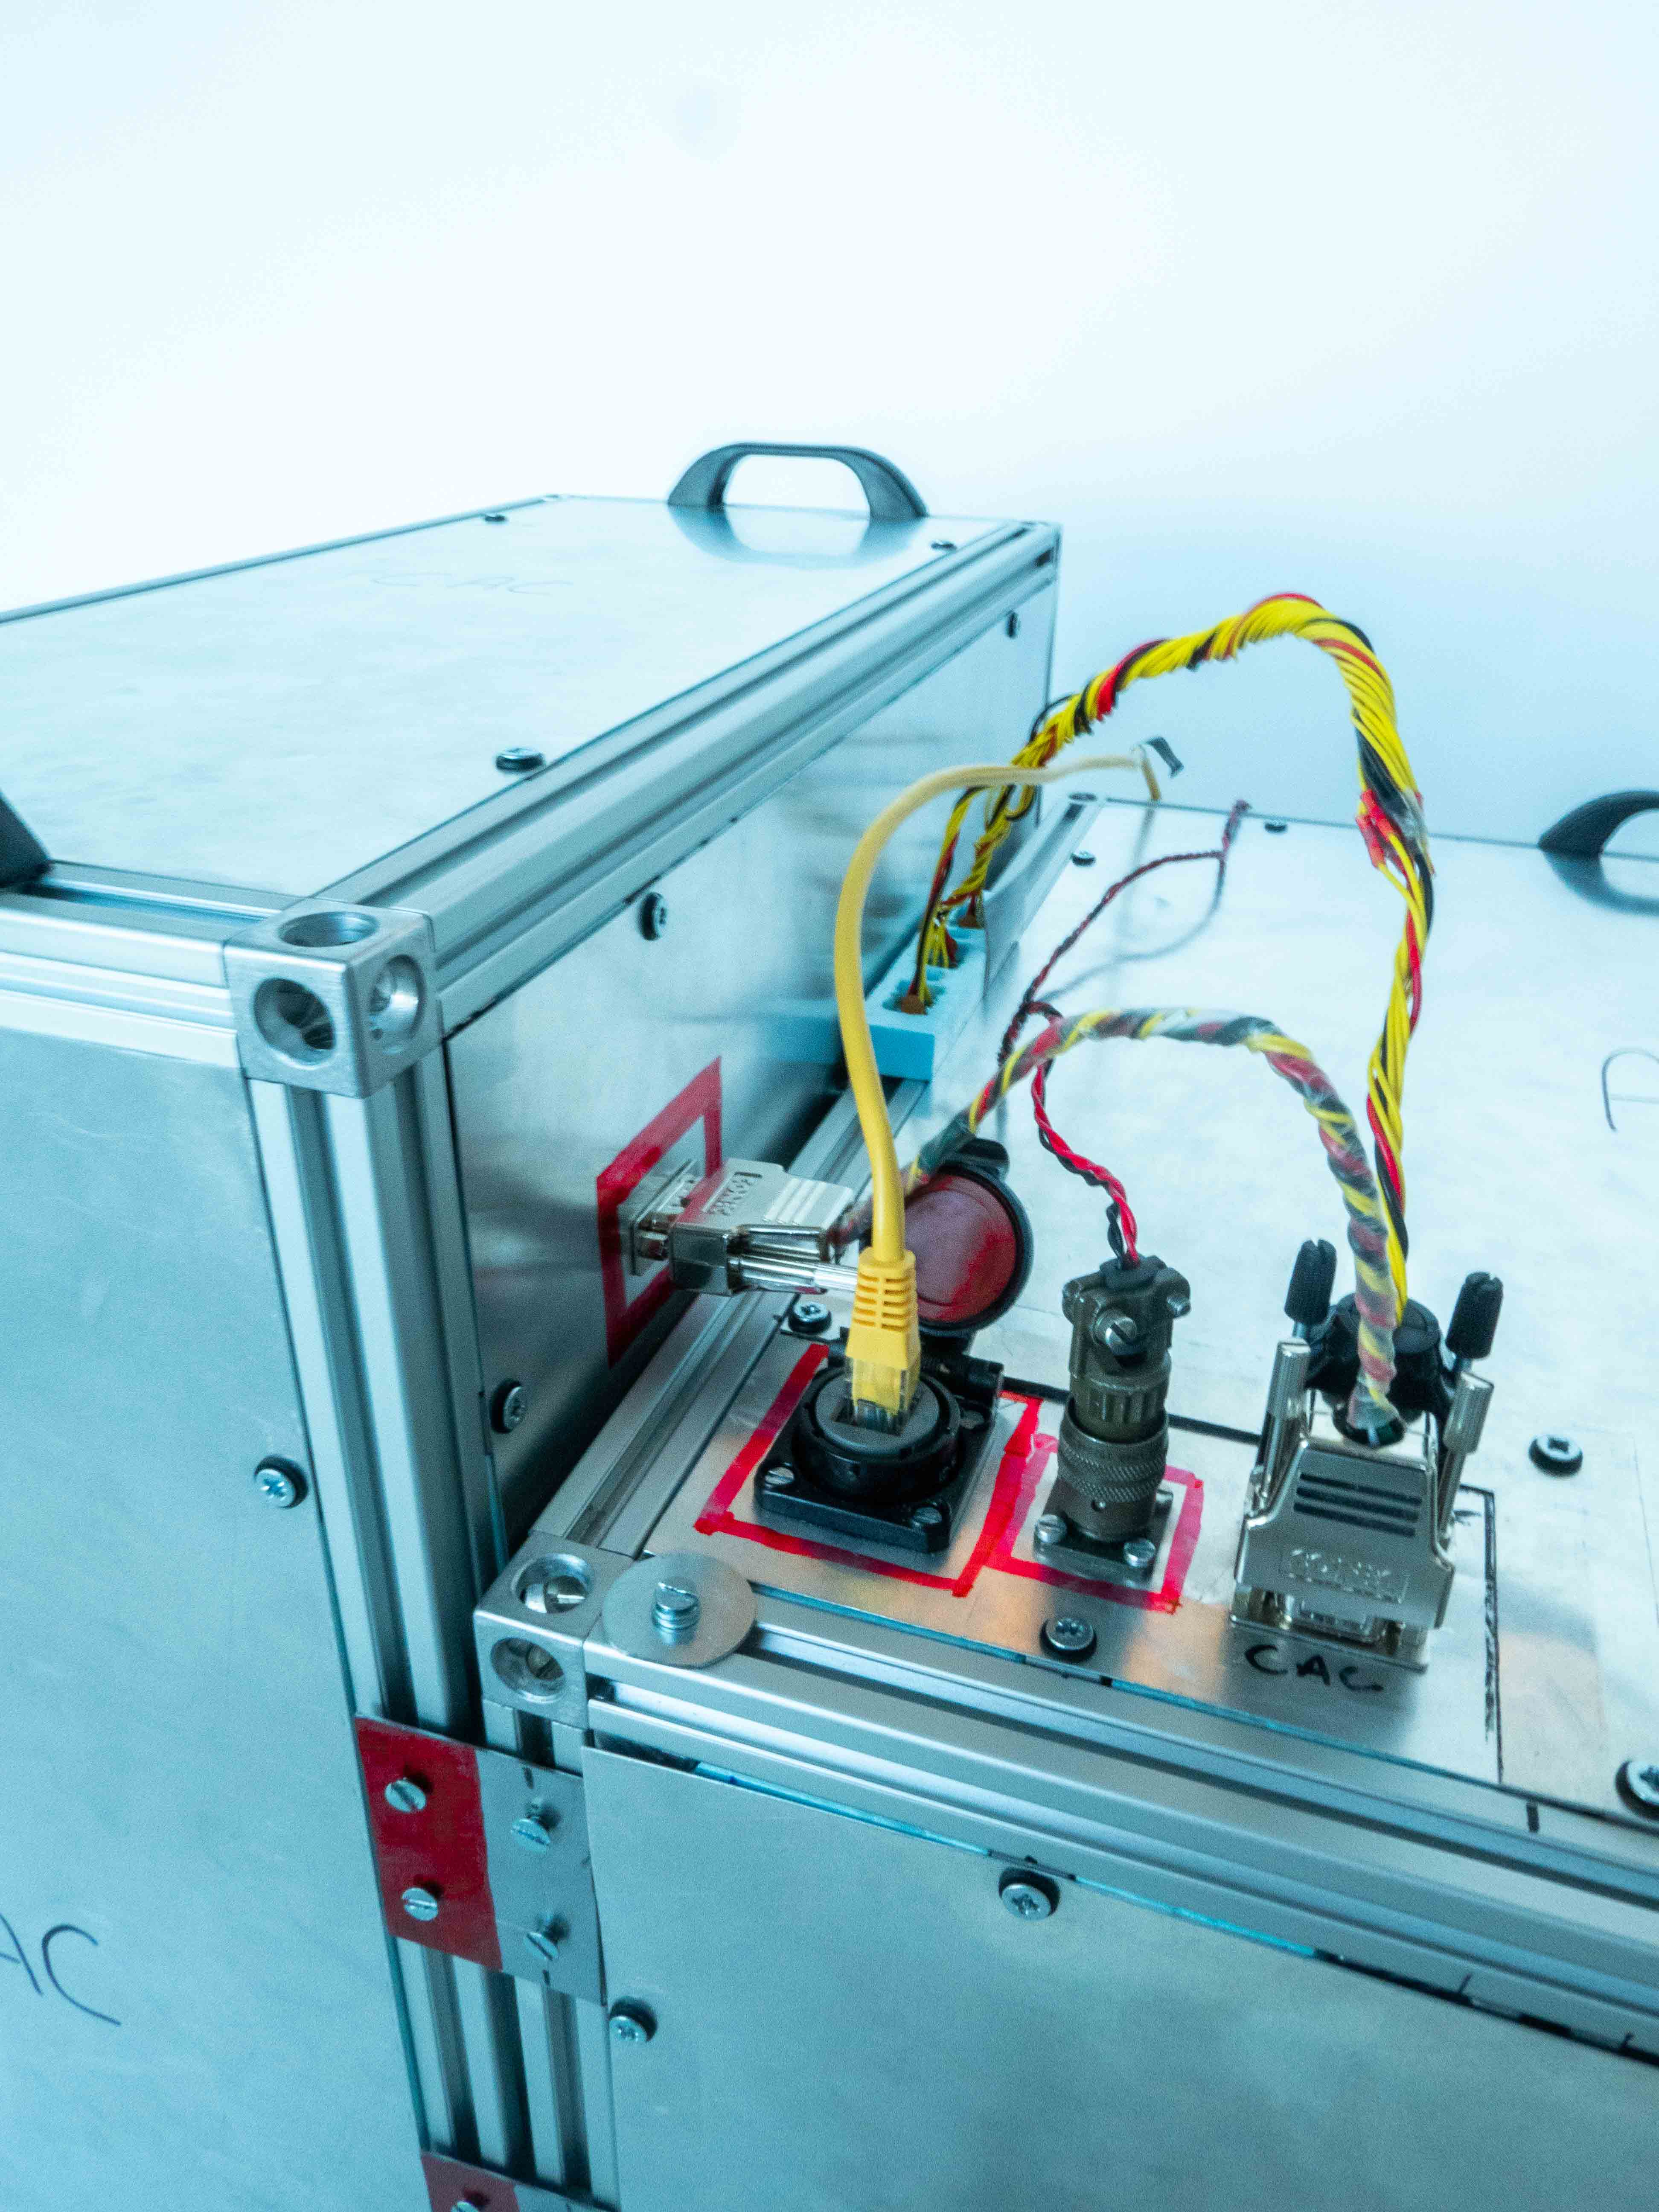
\includegraphics[width=0.5\textwidth]{appendix/img/Recovery_1.jpg}
    \caption{Electrical Interfaces detail.}
    \label{fig:Interfaces_Detail_I}
\end{figure}

\begin{figure}[H]
    \centering
    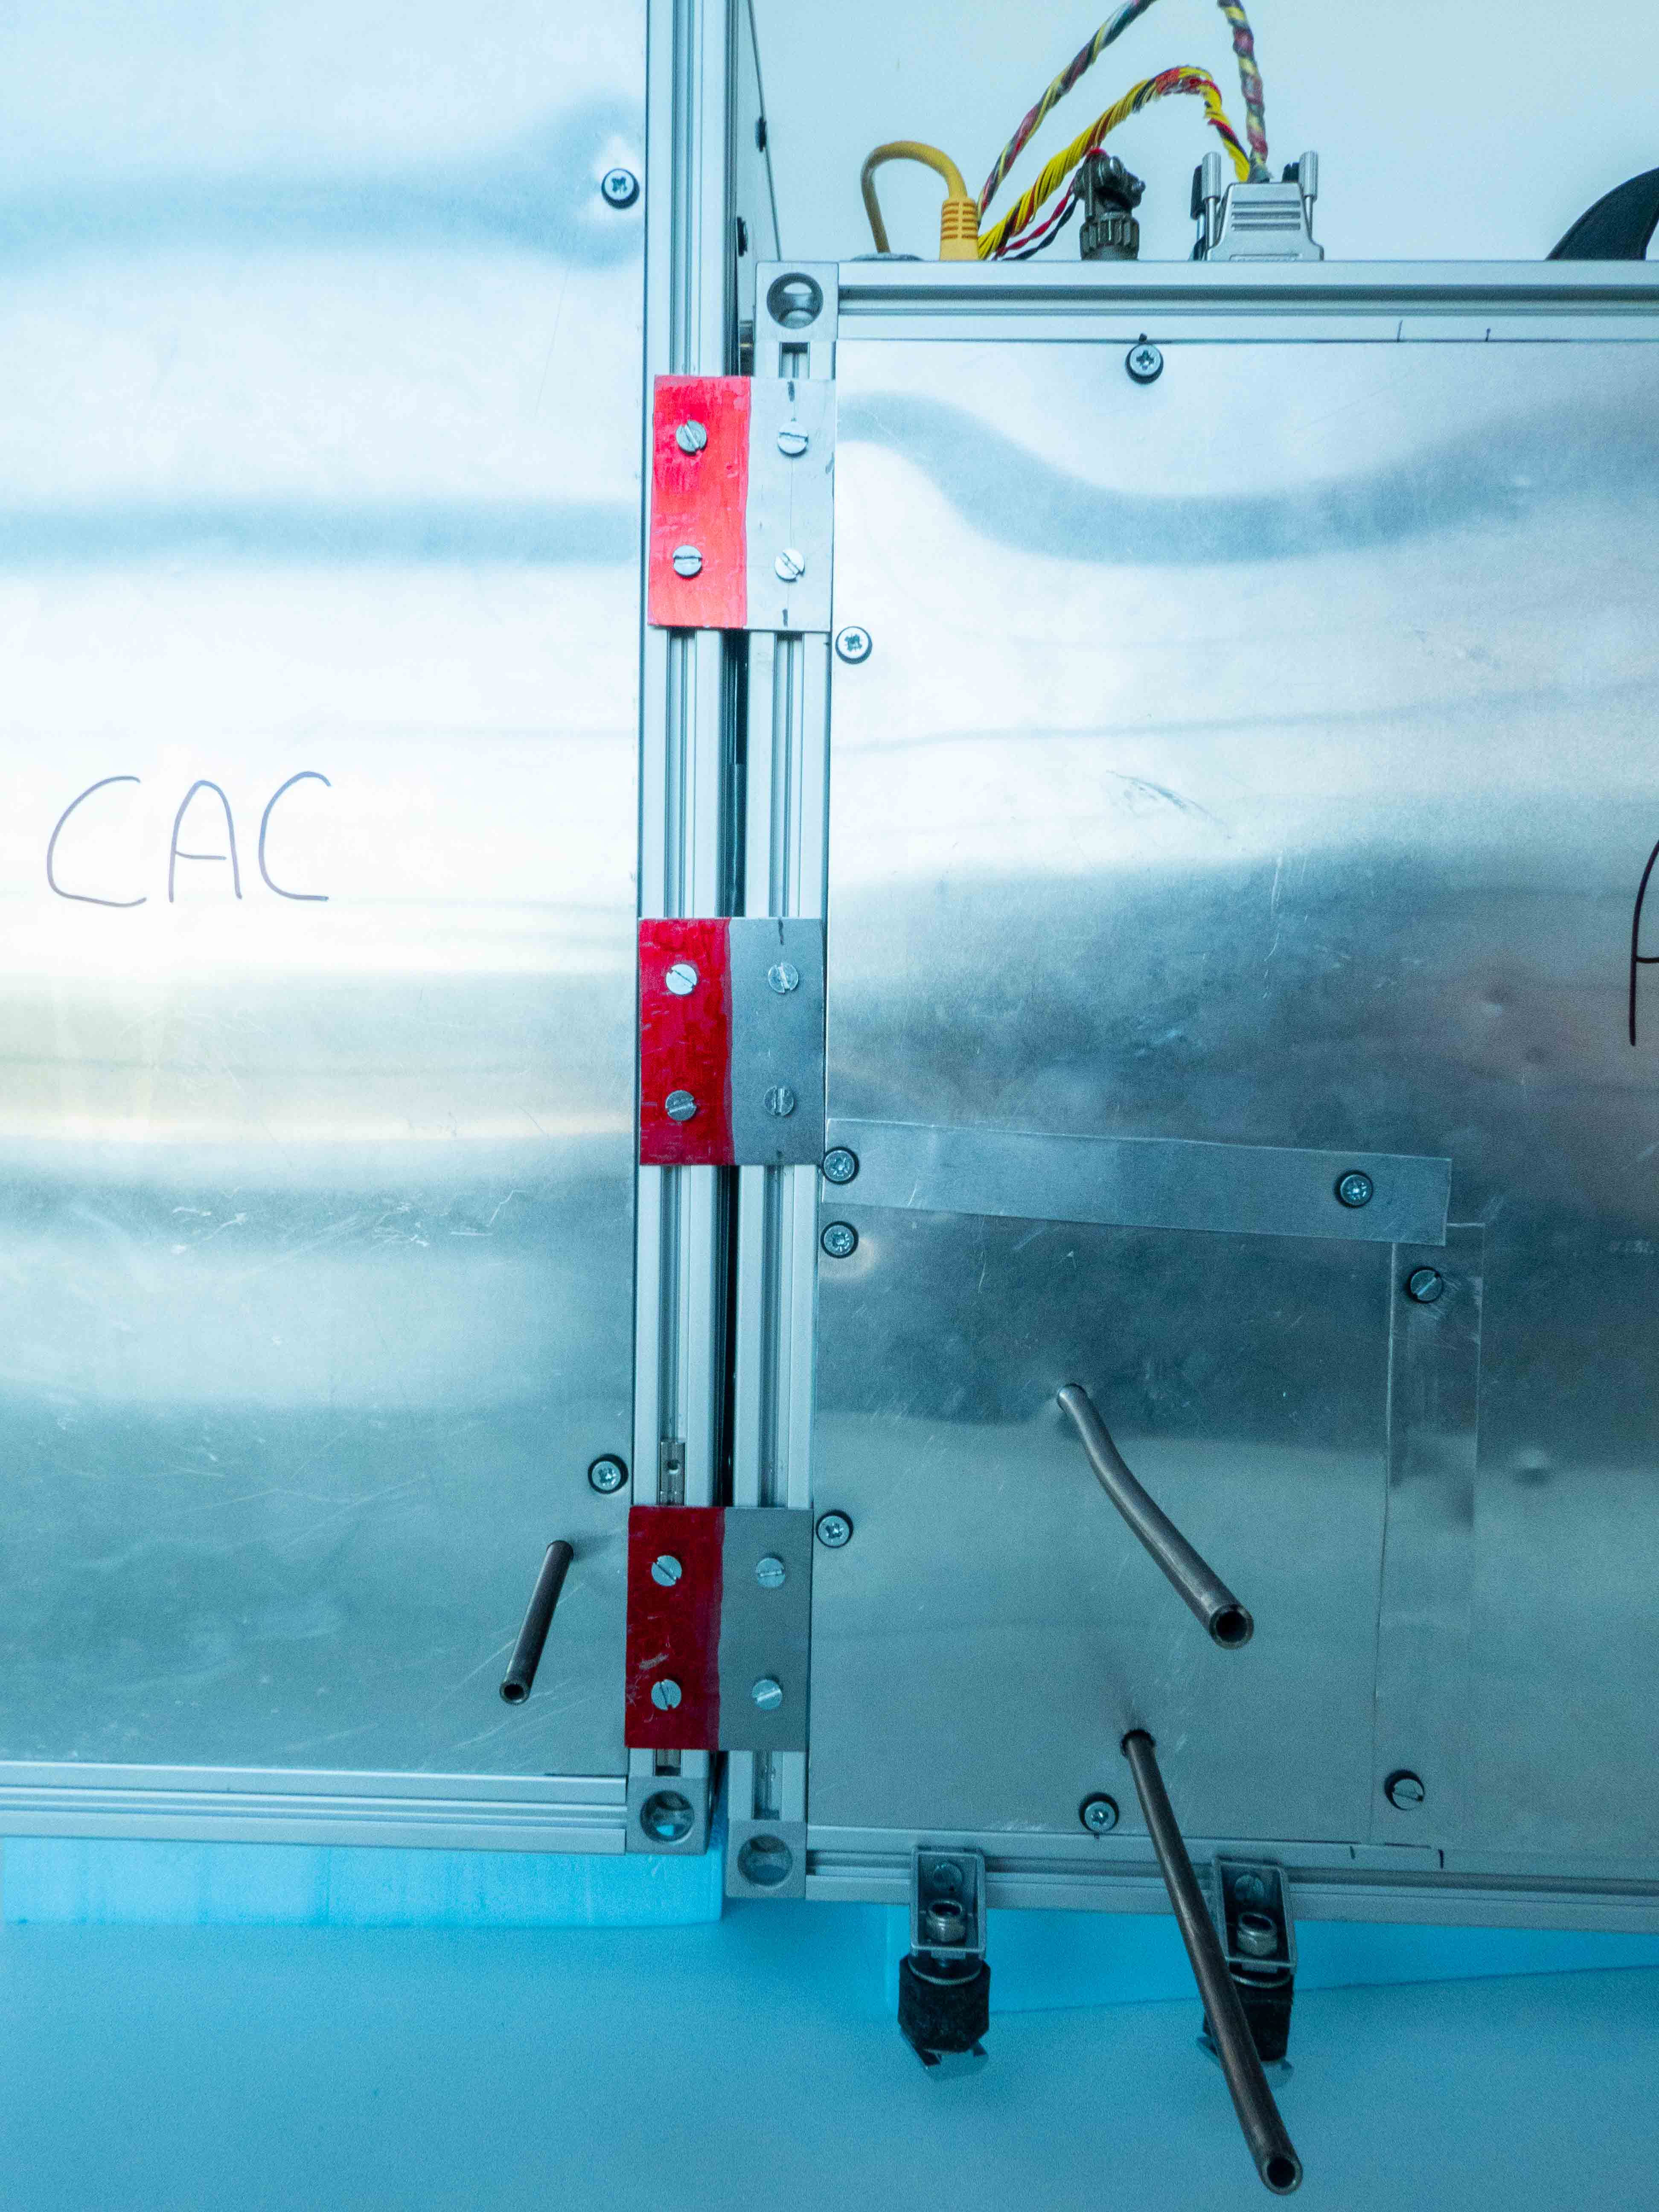
\includegraphics[width=0.5\textwidth]{appendix/img/Recovery_2.jpg}
    \caption{Fast Recovery Interfaces detail, boxes attachment.}
    \label{fig:Interfaces_Detail_II}
\end{figure}

\begin{figure}[H]
    \centering
    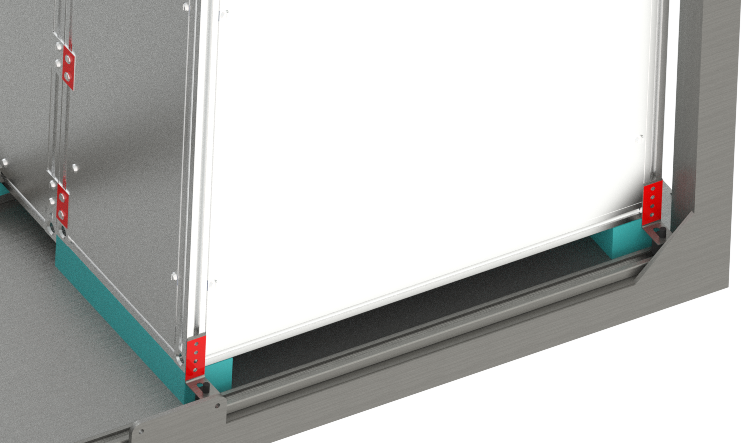
\includegraphics[width=0.7\textwidth]{appendix/img/Figure_49_Gondola_c.png}
    \caption{Fast Recovery Interfaces detail.}
    \label{fig:Interfaces_Detail_III}
\end{figure}

REGULAR RECOVERY OF AAC

\begin{itemize}
    \item Unscrew 8 gondola attachment points from the AAC.
    \item Remove the AAC Box from the gondola. Handles located at the top of the box. 
\end{itemize}

If the recovery is not nominal the following instructions should be followed. It should be noted that the chemical on-board, magnesium perchlorate, has the appearance of white powdery stones when dry and a white paste when wet.

\begin{itemize}
    \item If outer structure is damaged or white paste is seen in inlet tubes put on provided gloves before proceeding. Assume possibility chemicals are UNSAFE.
    \item If white paste is seen wipe with provided cloth and seal the end of tube with the provided plugs. Put any contaminated items into a bag which is then sealed.
    \item In event magnesium perchlorate comes into contact with skin wash immediately with water (following the MSDS procedure).
    \item In the event magnesium perchlorate comes into contact with clothes remove clothes as soon as possible and wash before wearing again.
    \item Even if no contact was made with the magnesium perchlorate it is recommended to wash hands after as a preventative measure.
    \item In the event that magnesium perchlorate is seen on the ground or inside the gondola, the appearance is a white paste or white stone, it should be recovered with gloves and wiped and placed into a sealed bag.
\end{itemize}

Provided material
\begin{itemize}
    \item Gloves
    \item Piece of cloth
    \item Plastic bag
    \item Three plugs
    \item Allen key set (at least \#3 and \#5)
    \item Clamp
\end{itemize}

\newpage

\newpage
%\raggedbottom
%\end{landscape}

